\documentclass[11pt,a4paper]{article}
\usepackage[margin=25mm]{geometry}
\usepackage[T1]{fontenc}
\usepackage{lmodern}
\usepackage{microtype}
\usepackage{amsmath,amssymb,booktabs,longtable,array}
\usepackage{xcolor}
\usepackage{hyperref}
\usepackage{listings}
\usepackage{enumitem}
\usepackage{graphicx}
\usepackage{tabularx}
\usepackage{placeins}
\hypersetup{colorlinks=true,linkcolor=blue!55!black,urlcolor=blue!55!black}
\graphicspath{{figures/}}
\lstset{basicstyle=\ttfamily\small,breaklines=true,frame=single,columns=fullflexible}
\setlist{nosep,leftmargin=*}
\title{Do Transformers Add Forecast Information?\\A Reproducible Comparison with Classical AR--GARCH}
\author{Solitons --- BITS Pilani\\\small Final empirical research report}
\date{21 November 2026}

\begin{document}
\maketitle
\begin{abstract}
The practical question is simple: when yesterday's return history is all that is known, does a
small Transformer improve tomorrow's S\&P 500 return forecast over predicting zero or fitting a
classical AR--GARCH model? We answer it with a chronological train/validation/test design,
one-step forecasts, fixed model parameters, and a single test evaluation after a committed
freeze. The analysis includes four Student-$t$ GARCH mean specifications, multi-proxy variance
scoring, a deliberately small PatchTST, validation-only forecast combinations, encompassing
regressions, and HAC Diebold--Mariano tests. PatchTST does not beat zero on validation (RMSE
1.2952 versus 1.1618 percentage points). A validation-fitted zero/training-mean combination
offers only a 0.0002-point RMSE gain over its best constituent. On the sealed test, classical
and simple forecasts are statistically indistinguishable under the predeclared primary test;
the frozen combination outperforms this PatchTST configuration. We also correct an
interpretation inherited from the project's initial log: standard GARCH persistence is
$\alpha+\beta$, whereas $\omega+\alpha+\beta$ is a scale-dependent registered diagnostic.
The evidence supports a narrow negative result for this asset, period, horizon, and model
configuration, not a general claim that Transformers cannot forecast returns.
\end{abstract}
\noindent\textbf{Keywords:} financial time series; AR--GARCH; PatchTST; forecast comparison;
volatility.
\tableofcontents
\newpage

\section{Research question and scope}
The project asks whether a Transformer adds useful conditional-mean forecast information beyond
classical AR/GARCH models, and whether forecast combinations improve predictive loss. It does not
assume the Transformer wins. The primary target is the next observed S\&P 500 daily log return.
The analysis does not claim trading profitability, predictability at other horizons, or universal
model rankings.

\subsection{Questions and hypotheses}
The empirical program separates four questions that should not be collapsed into a leaderboard:
\begin{enumerate}
\item Does the training sample contain detectable conditional-mean or conditional-variance
   structure? (EXP-001--004.)
\item Does the fixed PatchTST improve one-step conditional-mean forecasts on the validation
   dates shared with classical forecasts? The registered alternative was that PatchTST would
   have lower RMSE than every classical candidate; a failure to beat zero is a valid negative
   result (EXP-005--006.)
\item Does a convex combination estimated on validation improve on its constituents, and does
   either forecast add linear information conditional on another forecast? (EXP-007.)
\item Does the validation-frozen system retain its forecast performance on the sealed test
   sample? The primary null is equal expected squared forecast loss for the frozen combination
   and a comparator (EXP-008--009.)
\end{enumerate}
The decision rules are deliberately conservative. A lower likelihood information criterion is
not by itself evidence of better forecasting; a lower point RMSE is not by itself evidence of a
statistical difference; and the validation minimum is subject to selection optimism.

\subsection{Why compare these model families?}
The AR--GARCH family makes a transparent decomposition: a small linear conditional mean and a
time-varying conditional variance. Student-$t$ innovations allow heavier tails than a Gaussian
likelihood. PatchTST represents the recent series as overlapping patches and lets attention
combine information across those patches. The original PatchTST design emphasizes patching and
channel independence; this project uses only a small univariate one-step head, not the full range
of long-horizon configurations in the original paper. The comparison is therefore between a
specified small neural baseline and established low-parameter return/volatility models, not a
claim to reproduce every published architecture.

The work is an empirical audit as much as a model comparison: the common origins, target units,
preprocessing boundary, validation-only weights, convergence records, and freeze manifest make
the reasoning behind a negative result inspectable. The complete source citations appear at the
end of this report.

\subsection{Data, units, and chronological split}
The raw source is \path{data/raw/sp500.csv}; processed observations are in
\path{data/processed/sp500_returns.csv}. The price field is \texttt{Close}; the stored target
is
\begin{equation}
 r_t=100\log(C_t/C_{t-1}).
\end{equation}
Thus $r_t$ is a percentage-point log return. The column \texttt{log\_return} is the same change
in decimal units, so $r_t=100\,\texttt{log\_return}_t$. Squared-return variance is in
percentage-point squared units. The provenance tests confirm raw/processed close agreement,
return identities, OHLC constraints, finite values, date order, uniqueness, and row counts.

\begin{center}
\begin{tabular}{llll}
\toprule
Partition & $n$ & First observation & Last observation\\
\midrule
Train & 2,815 & 2010-01-05 & 2021-03-11\\
Validation & 603 & 2021-03-12 & 2023-08-03\\
Test & 604 & 2023-08-04 & 2025-12-30\\
\bottomrule
\end{tabular}
\end{center}
Observations are never randomly shuffled. Actual exchange trading dates are retained; no regular
calendar frequency is fabricated. The provenance check establishes weekday-only dates, not a
separate exchange-holiday calendar match.

\begin{figure}[htbp]
\centering
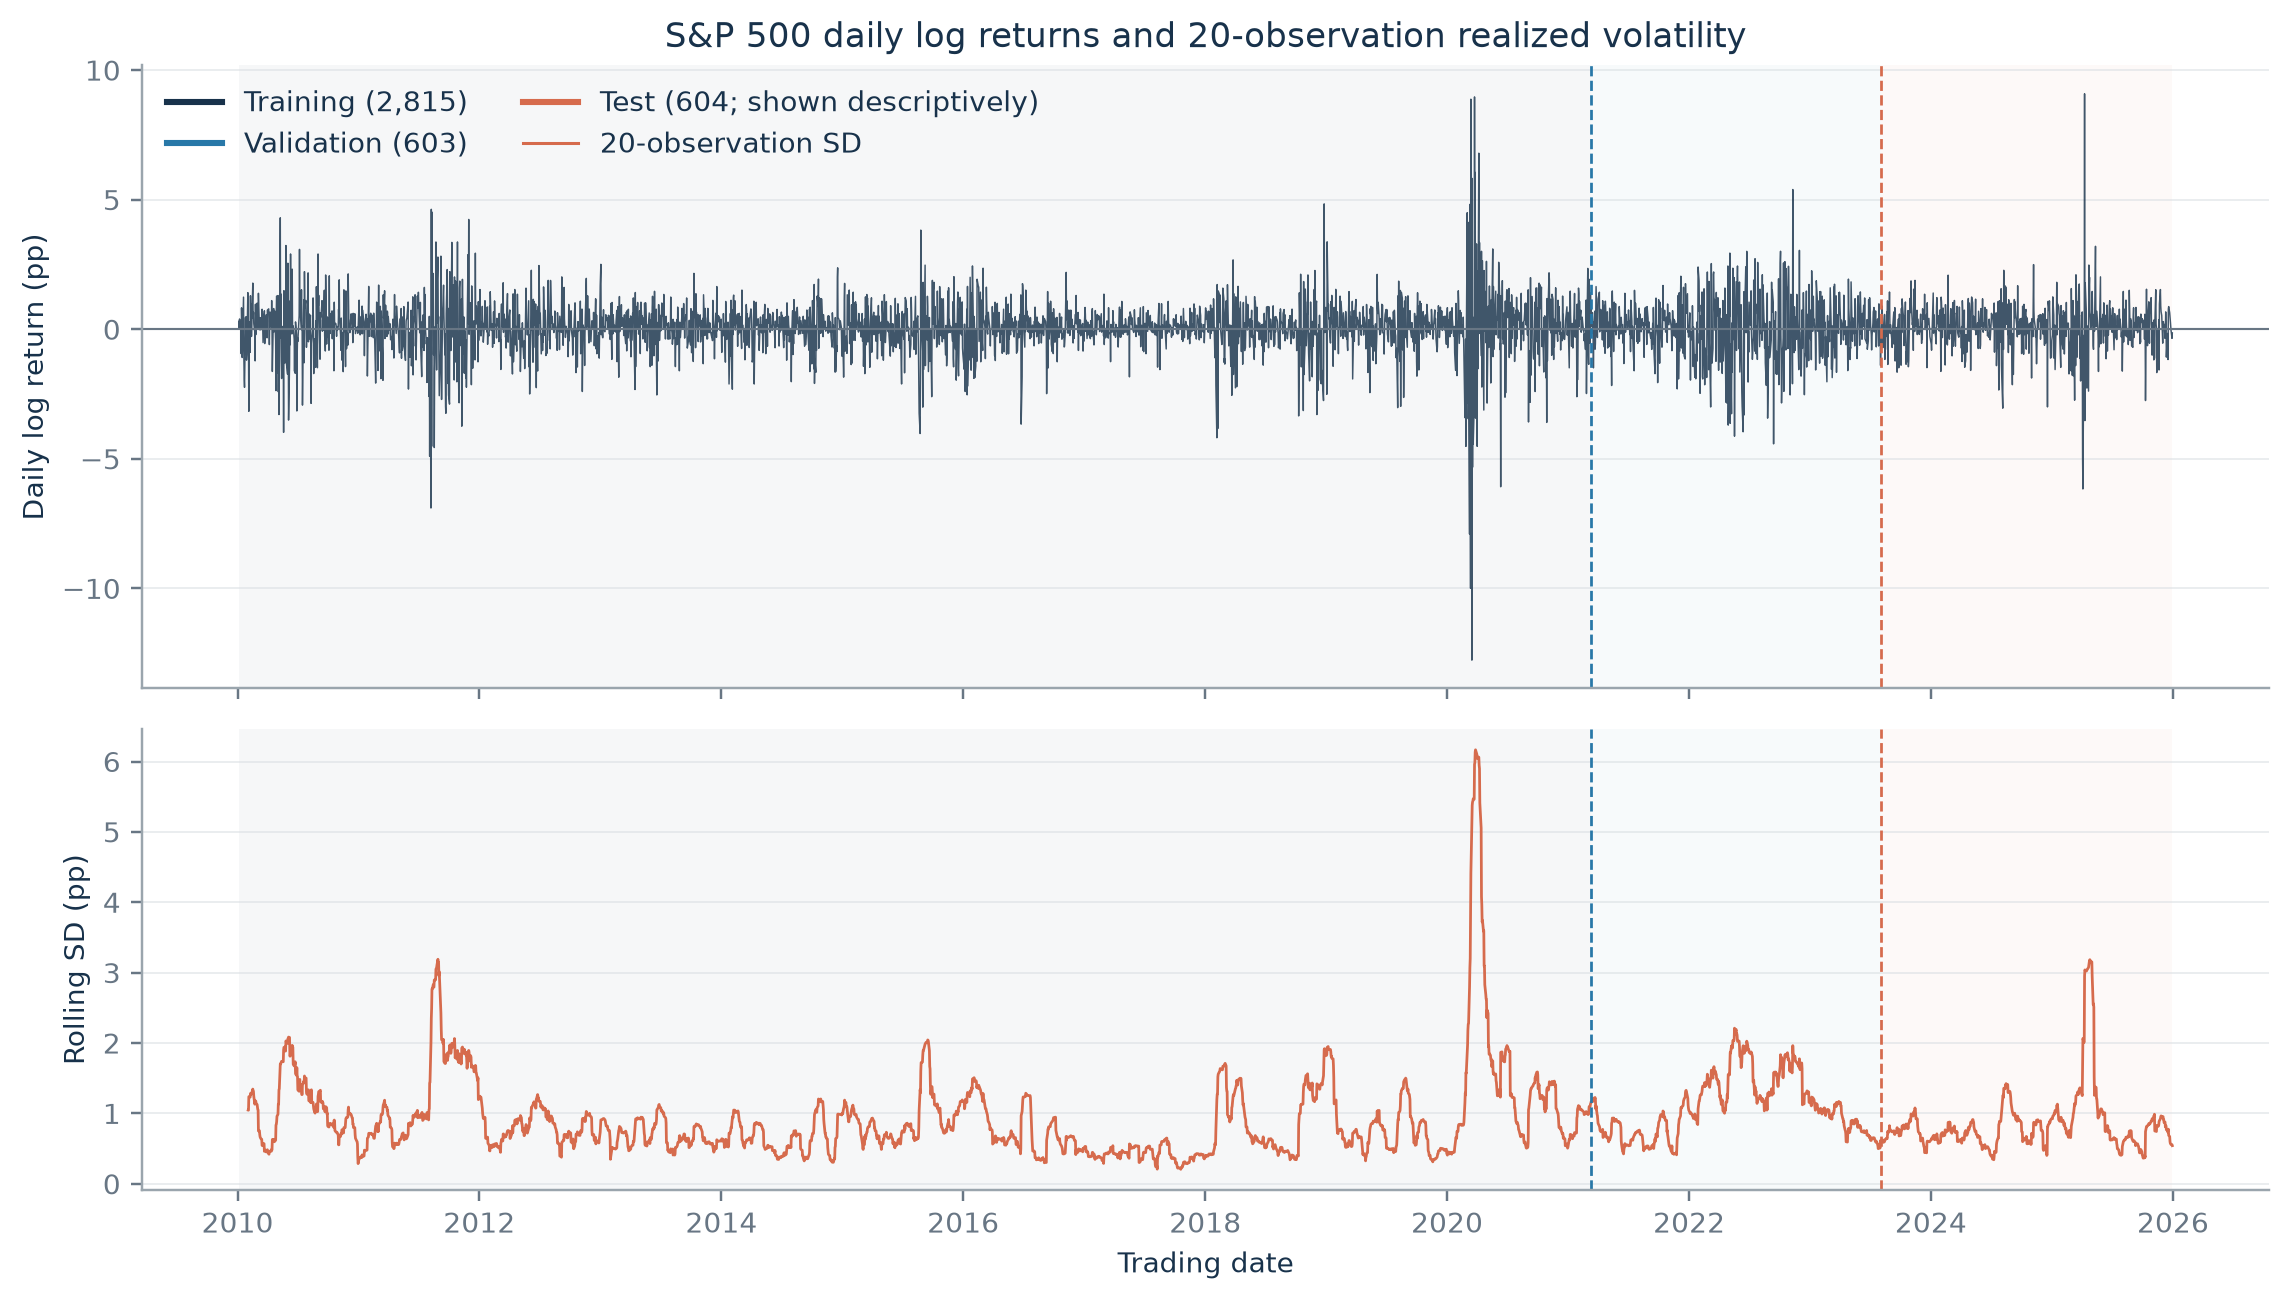
\includegraphics[width=0.98\linewidth]{fig1_returns_volatility.png}
\caption{Observed daily returns and trailing 20-observation standard deviation. Dashed lines
mark train/validation and validation/test boundaries. The test segment is displayed only as an
ex-post description after the one-time EXP-009 evaluation; it did not enter model fitting or
selection. Volatility clusters are visible: large absolute returns tend to occur in groups.}
\label{fig:returns-volatility}
\end{figure}
Figure~\ref{fig:returns-volatility} shows why a constant-variance model is a weak benchmark:
the scale of returns varies markedly over time. It also shows why a return-level forecasting
problem is difficult: most observations remain close to zero, while a relatively small number of
large moves dominate squared-error loss.

\begin{figure}[htbp]
\centering
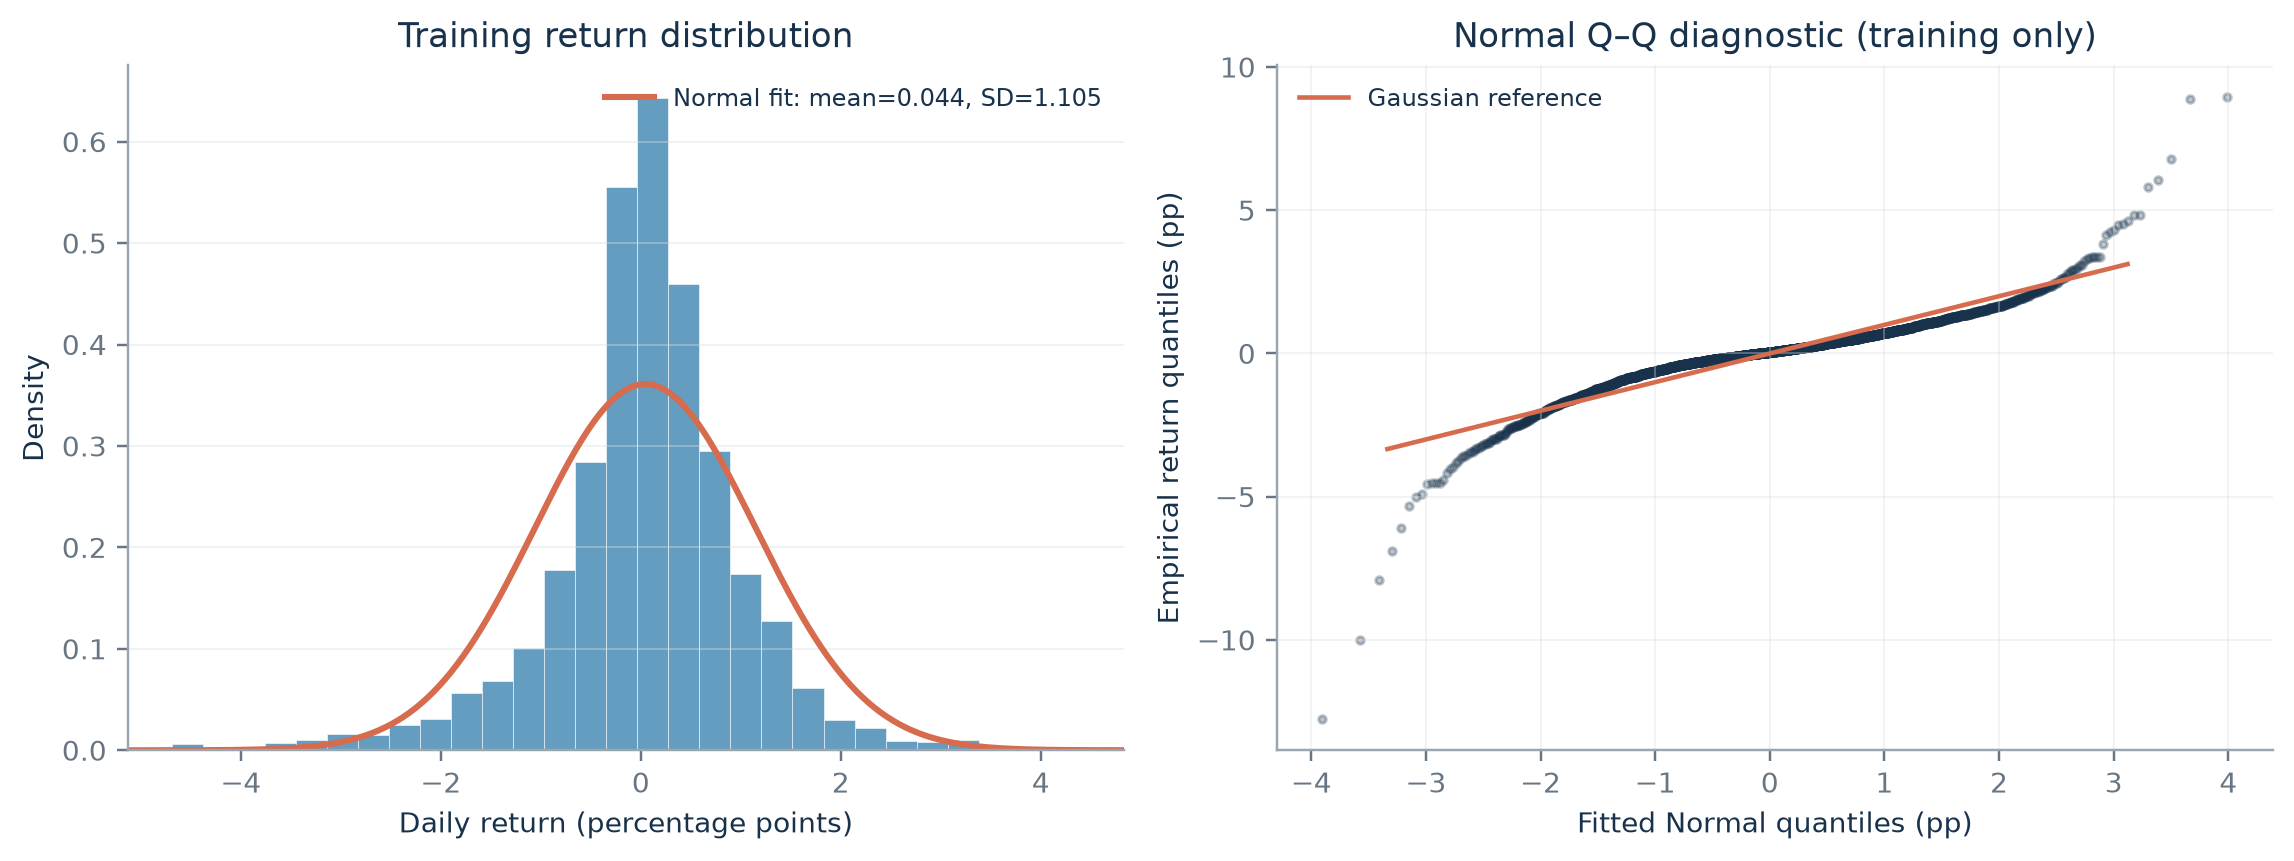
\includegraphics[width=0.98\linewidth]{fig2_train_distribution.png}
\caption{Training return distribution against a fitted Gaussian with the same training mean and
standard deviation, plus the corresponding normal Q--Q diagnostic. Extreme empirical quantiles
depart from the reference line, consistent with the training excess kurtosis of 16.15 and the
Student-$t$ innovation choice. The plot is fit and drawn from training observations only.}
\label{fig:train-distribution}
\end{figure}

\subsection{Forecast protocol}
At each validation or test origin $t$, forecast $r_t$ using information available before that
return is revealed. After the observation becomes known it may enter the next origin's history.
Classical parameter estimates and PatchTST weights stay fixed after training. The Transformer
scaler is fit on the training partition only. Candidate forecasts are compared on the same dates
and one-step horizon. Test outcomes were kept sealed until \texttt{docs/freeze\_manifest.json}
had been committed as \texttt{6fb7b57}.

\section{Experiments completed}
\begin{longtable}{>{\raggedright\arraybackslash}p{0.12\linewidth}>{\raggedright\arraybackslash}p{0.29\linewidth}>{\raggedright\arraybackslash}p{0.49\linewidth}}
\toprule
ID & Objective & Result/status\\
\midrule
EXP-000 & Check data provenance and trading dates. & Completed in substance; automated identities pass. No external holiday-calendar cross-check.\\
EXP-001 & Assess stationarity and dependence. & Training-only ADF rejects a unit root; squared-return ARCH LM strongly rejects homoskedasticity.\\
EXP-002 & Score ARIMA means versus simple baselines. & No dynamic candidate beats the zero/training-mean baselines on validation.\\
EXP-003 & Compare four GARCH(1,1)-Student-$t$ mean specifications. & All fit; validation mean RMSE favors zero very slightly. Persistence estimates exceed one.\\
EXP-004 & Evaluate variance forecasts using multiple proxies. & GARCH beats constant variance; EWMA is competitive or better depending on proxy.\\
EXP-004-S1 & Constrain persistence below one. & Boundary solutions; a small AR(1)/AR(2) QLIKE ordering swap requires a scoped qualification.\\
EXP-005 & Train one small univariate PatchTST. & Validation RMSE 1.2952 versus 1.1618 for zero; hypothesis rejected.\\
EXP-006 & Compare on identical validation dates. & PatchTST loses to all simple/classical mean candidates by RMSE.\\
EXP-007 & Fit convex combination weights and encompassing regressions on validation. & Zero + training mean is the best pair, but its RMSE gain is only 0.000211.\\
EXP-008 & Apply HAC DM tests to paired validation losses. & Baselines strongly outperform PatchTST in validation; other model differences are small.\\
EXP-009 & One sealed confirmatory test. & Frozen combination is not statistically distinguishable from classical means; it outperforms PatchTST.\\
\bottomrule
\end{longtable}

\section{Concepts and equations}
\subsection{Conditional mean and GARCH variance}
The classical model separates expected return from its shock:
\begin{align}
 r_t &= \mu_t+\epsilon_t, & \epsilon_t&=\sigma_t z_t,\\
 \sigma_t^2&=\omega+\alpha\epsilon_{t-1}^2+\beta\sigma_{t-1}^2,
 & z_t&\sim t_\nu\text{ standardized},
\end{align}
with $\omega>0$, $\alpha,\beta\geq0$, and degrees of freedom $\nu>2$. The innovation is
Student-$t$ to allow heavier tails than a Gaussian model. Mean candidates are zero, constant,
AR(1), and AR(2):
\begin{align}
\mu_t&=0,\quad \mu,\quad \mu+\phi_1r_{t-1},\quad
\mu+\phi_1r_{t-1}+\phi_2r_{t-2}.
\end{align}
The recursion implies a variance shock decays at a rate governed by $\alpha+\beta$. Under the
standard GARCH(1,1) assumptions, a finite unconditional variance exists when
\begin{equation}
 \alpha+\beta<1,\qquad \operatorname{Var}(\epsilon_t)=\frac{\omega}{1-\alpha-\beta}.
\end{equation}
This condition is distinct from strict stationarity of every possible GARCH process, but is the
usual finite-second-moment condition relevant to unconditional variance. Here $\omega$ has
return-squared units, while $\alpha$ and $\beta$ are dimensionless. The historical project log
also called $\omega+\alpha+\beta$ ``persistence''; that sum changes when return units change and
is not the canonical persistence measure. We retain it in the results as a registered diagnostic
and report $\alpha+\beta$ separately. This distinction matters: the unconstrained fits have
$\alpha+\beta$ just below one, although $\omega+\alpha+\beta$ is slightly above one.

The four EXP-003 fits used \texttt{hold\_back=2}; all likelihoods therefore use 2,813 of the
2,815 training observations. A common effective sample is necessary for within-family
information-criterion comparisons. AIC/BIC are not compared across unlike likelihood
implementations, and AIC alone did not select the forecasting model.

\begin{table}[htbp]
\centering\small
\caption{EXP-003 training likelihood, model coefficients of interest, and validation mean error.}
\label{tab:garch-specifications}
\begin{tabular}{lrrrrrrr}
\toprule
Mean & $\ell$ & AIC & $\alpha+\beta$ & $\omega+\alpha+\beta$ & $p_{LB,z}(20)$ & $p_{LB,z^2}(20)$ & RMSE\\
\midrule
Zero & $-3458.99$ & 6925.98 & 0.99085 & 1.01643 & 0.153 & 0.812 & 1.16180\\
Constant & $-3429.71$ & 6869.43 & 0.99336 & 1.02005 & 0.092 & 0.861 & 1.16370\\
AR(1) & $-3423.88$ & 6859.76 & 0.99410 & 1.02001 & 0.080 & 0.862 & 1.16689\\
AR(2) & $-3423.84$ & 6861.68 & 0.99412 & 1.01999 & 0.078 & 0.863 & 1.16660\\
\bottomrule
\end{tabular}
\begin{minipage}{0.96\linewidth}\footnotesize
All candidates converged; effective sample $n=2,813$. The standardized-residual ARCH LM(10)
$p$-values were 0.565, 0.654, 0.666, and 0.668 for zero, constant, AR(1), and AR(2), respectively.
The Ljung--Box columns report lag-20 $p$-values. The last column is validation RMSE in percentage
points. These are fit diagnostics and forecasts, not proofs of correct specification.
\end{minipage}
\end{table}
The training AIC minimum is AR(1), but zero mean has the lowest validation RMSE among the four
GARCH specifications. The point differences are small; the registered validation baselines are
slightly better still. This is the concrete reason the report does not treat AIC as a forecast
selection rule.

\paragraph{Numerical GARCH example.} Using the zero-mean fit's approximate parameters
$\omega=0.02558$, $\alpha=0.173$, $\beta=0.818$, suppose the previous shock is $0.5$ percentage
points and previous conditional variance is $1.2$ percentage-point$^2$. Then
\[
 \widehat\sigma_t^2=0.02558+0.173(0.5)^2+0.818(1.2)\approx1.0505.
\]
This is a variance forecast; its square root is about $1.025$ percentage points of daily
conditional standard deviation.

\subsection{Residual diagnostics and variance loss}
The ADF null is a unit root. Ljung--Box tests assess residual autocorrelation through a selected
lag. Engle's ARCH LM null is no conditional heteroskedasticity through the tested lag. A small
$p$-value is evidence against the null, not a measure of forecast accuracy.

For a variance forecast $\hat v_t>0$ and a proxy $q_t$, EXP-004 uses QLIKE:
\begin{equation}
 L_{Q,t}=q_t/\hat v_t+\log\hat v_t,\qquad
 \overline L_Q=T^{-1}\sum_t L_{Q,t}.
\end{equation}
The squared return $q_t=r_t^2$ is a noisy variance proxy. Intraday Parkinson range and an EWMA
smoothed proxy are also used. QLIKE levels are compared only within a proxy column because the
proxies have different scales and noise. Parkinson's decimal-squared variance is converted to
percentage-point-squared units by multiplying by $10^4$. The EWMA proxy uses current $r_t^2$;
the one-step EWMA forecast uses only $r_{t-1}^2$.

\paragraph{Numerical QLIKE example.} If $r_t^2=1$ and the forecast is $\hat v_t=1.05$, the loss
is $1/1.05+\log(1.05)\approx1.0012$. Both terms must use squared-return units.

\subsection{Box--Jenkins identification, estimation, and diagnostic checking}
A supplementary Box--Jenkins screen was run using the training partition only. The sequence is
identification, estimation, and diagnostic checking. First, the ADF test on the 2,815 training
returns rejects a unit root (statistic $-11.7049$, $p=1.54\times10^{-21}$). ACF and PACF plots
are useful identification aids, but they do not mechanically determine an order. To make the
screen reproducible, candidate ARIMA$(p,0,q)$ models with a constant were fitted for
$p,q\in\{0,1,2,3\}$ and ranked by AICc. The minimum AICc is obtained by ARMA$(2,2)$:
AIC $=8404.261$, BIC $=8439.917$, and AICc $=8404.291$.

The selected screening model is then estimated on the same training partition and its residuals
are checked. The Ljung--Box tests use the fitted-model degrees-of-freedom adjustment
$\texttt{model\_df}=p+q=4$. The lag-10 statistic is $25.712$ ($p=0.000252$) and the lag-20
statistic is $41.492$ ($p=0.000470$), rejecting residual whiteness at both lags. Engle's ARCH
LM statistic at 10 lags is $877.423$ ($p=4.60\times10^{-182}$), rejecting constant conditional
variance. The Jarque--Bera statistic is $15174.5$; its computed $p$-value underflows to zero,
consistent with pronounced non-normality.

This ARMA$(2,2)$ is a supplementary mean-model screen, not the final forecast model and not a
replacement for the registered AR--GARCH comparisons. The remaining residual autocorrelation and
very strong ARCH effect show that a mean-only ARMA model is incomplete for these returns. The
result motivates conditional-variance modelling and heavy-tailed innovations. The exact candidate
grid and diagnostic output are saved in
\path{results/tables/box_jenkins_training_diagnostics.json}; the reproducible script is
\path{src/classical/box_jenkins.py}. The validation and test partitions are not read by this
screen.

\subsection{PatchTST and scaling}
PatchTST divides the trailing lookback into overlapping patches, embeds the patches, applies
self-attention, then maps the encoded sequence to one forecast. With lookback $L$, patch length
$p$, and stride $s$, the token count is
\begin{equation}
 P=\left\lfloor\frac{L-p}{s}\right\rfloor+1.
\end{equation}
EXP-005 set $L=96$, $p=16$, $s=8$, giving $P=11$ patches, $d_{model}=64$, four attention
heads, two encoder layers, feed-forward size 128, and 69,441 trainable parameters. Adam uses
learning rate $10^{-3}$, weight decay $10^{-4}$, batch size 64, dropout 0.1, and seed 42 on CPU.
The loss is mean squared error on scaled targets. Early stopping uses an internal 15\% tail
inside training, then a fresh model is trained on all training windows for the selected ten epochs.

The two phases are important for interpretation. Phase 1 uses 2,296 training windows and 423
internal-validation target windows to choose the epoch. Phase 2 starts from a fresh seeded
initialization and uses all 2,719 training windows for ten epochs. The registered validation
partition is not used for model selection. Window minibatches retain chronological order to
honor the project no-shuffling rule.

The train-only transformation is
\[
 z_t=(r_t-\bar r_{train})/s_{train},\qquad
 \hat r_t=s_{train}\hat z_t+\bar r_{train}.
\]
Here $\bar r_{train}=0.04427$ and $s_{train}=1.10524$ percentage points. For a scaled prediction
of 0.20, the returned forecast is $0.04427+1.10524(0.20)=0.2653$ percentage points. A forecast
window for origin $t$ contains observations $t-96,\ldots,t-1$ and never the target itself.

\begin{figure}[htbp]
\centering
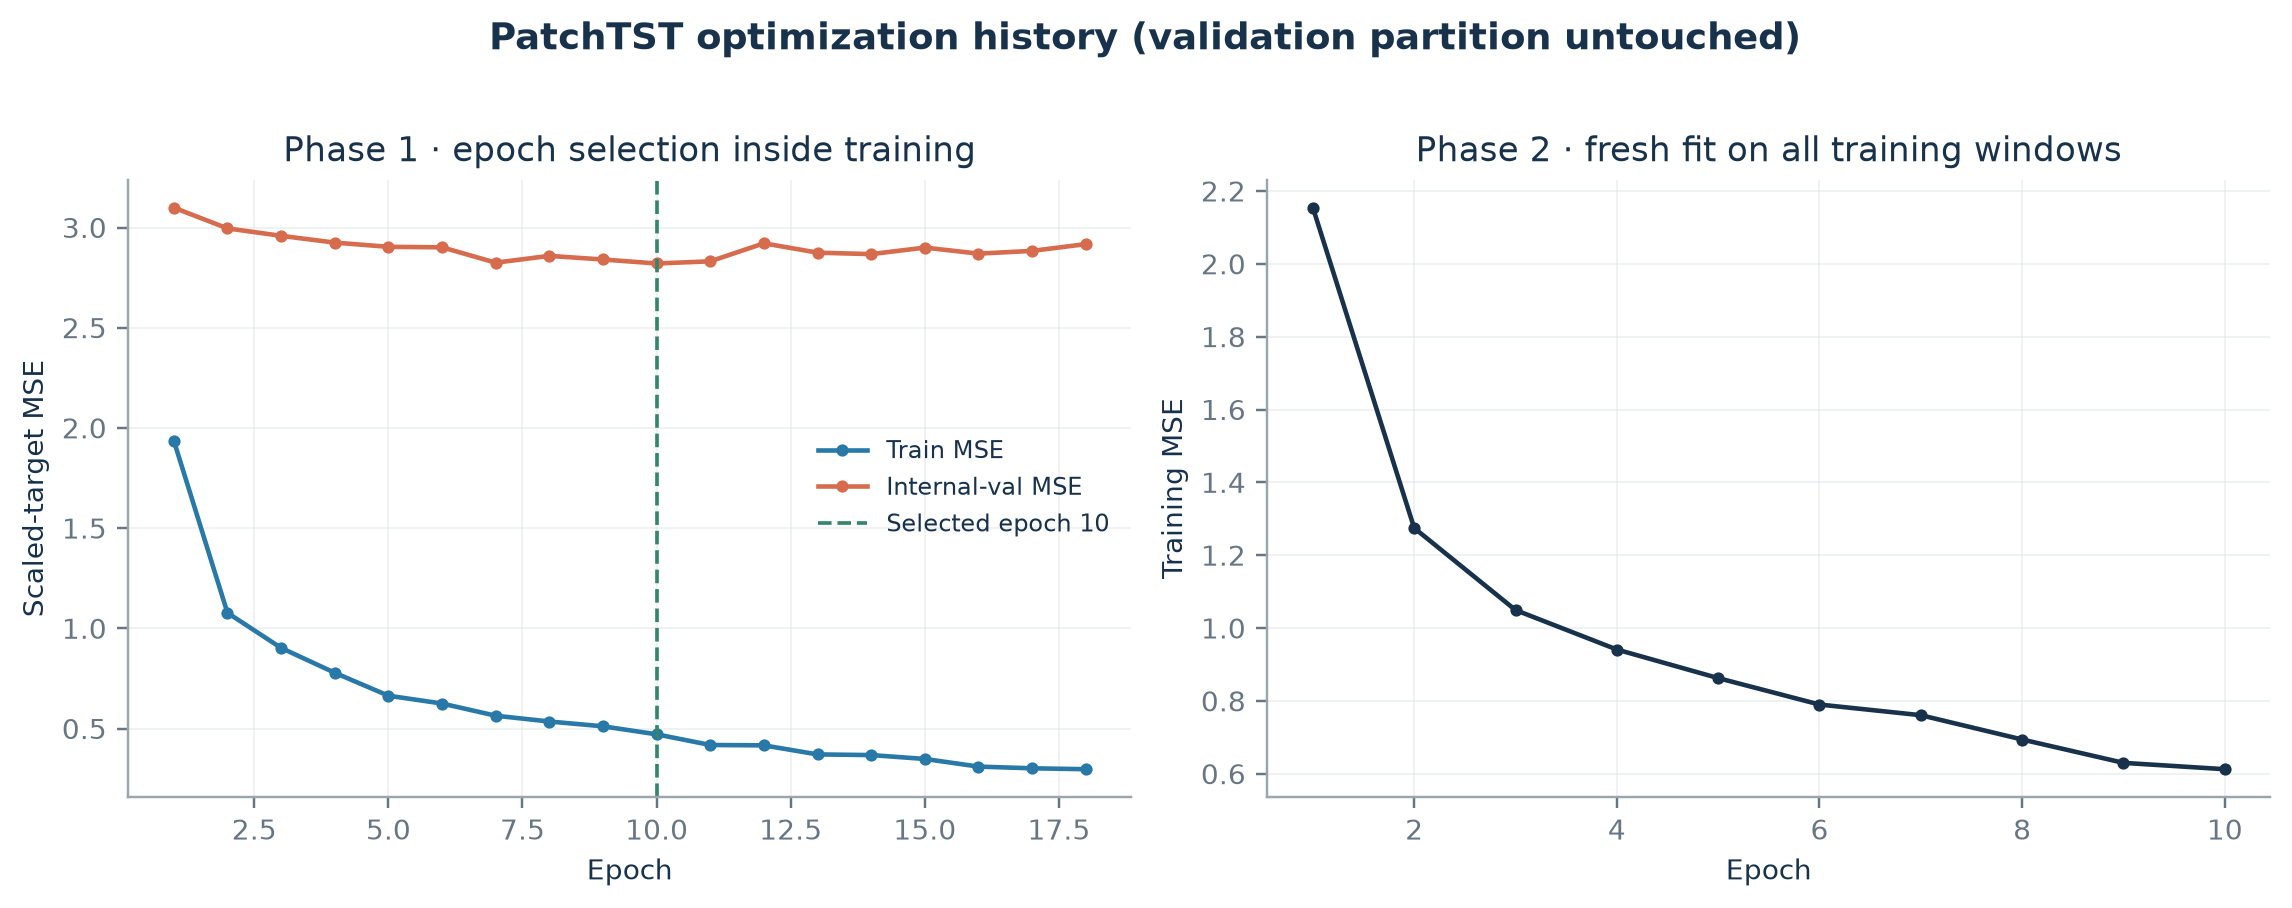
\includegraphics[width=0.98\linewidth]{fig5_patchtst_learning_curves.png}
\caption{Training and internal-validation MSE used for PatchTST epoch selection, followed by a
fresh Phase 2 fit on the full training partition. The minimum internal-validation MSE occurs at
epoch 10. The registered validation sample is not plotted here and did not select the epoch.}
\label{fig:patchtst-learning}
\end{figure}

\subsection{Forecast combinations and encompassing}
For forecasts $f_A$ and $f_B$, a convex combination is
\begin{equation}
 f_t(w)=wf_{A,t}+(1-w)f_{B,t},\qquad 0\leq w\leq1.
\end{equation}
The validation-SSE minimizer is
\begin{equation}
 w^*=\operatorname{clip}_{[0,1]}
 \frac{\sum_t(f_{A,t}-f_{B,t})(y_t-f_{B,t})}
 {\sum_t(f_{A,t}-f_{B,t})^2}.
\end{equation}
The weights are fitted on validation only, then frozen. The encompassing regression
\begin{equation}
 y_t=c+b_Af_{A,t}+b_Bf_{B,t}+u_t
\end{equation}
tests whether a forecast adds conditional linear signal. Newey--West HAC standard errors allow
short-range serial dependence. If a forecast is constant, it is collinear with the intercept;
the coefficient is not identified, so the code records that status rather than reporting a
misleading value.

\paragraph{Numerical combination example.} The validation fit assigns weights 0.499943 to zero
and 0.500057 to the training mean (0.044268). Its constant forecast is about
$0.500057(0.044268)=0.02214$ percentage points. RMSE moves from 1.161796 to 1.161585, a gain
of 0.000211. This tiny gain is expected to be optimistic because the same validation sample
chooses and scores the weight.

\subsection{Diebold--Mariano test}
For model A and B define a loss differential $d_t=L(e_{A,t})-L(e_{B,t})$. The null is
$E[d_t]=0$. Negative mean $d_t$ favors A. The statistic is
\begin{equation}
 DM=\frac{\bar d}{\sqrt{\widehat\Omega/T}},
\end{equation}
where $\widehat\Omega$ is a Bartlett Newey--West estimate of long-run variance. The HAC
bandwidth is selected by
\begin{equation}
 b=\left\lfloor4(T/100)^{2/9}\right\rfloor,
\end{equation}
which equals five for both evaluation windows. At horizon $h=1$, the HLN adjustment is
\begin{equation}
 c_1^2=1-1/T,\qquad DM_{HLN}=c_1DM.
\end{equation}
A two-sided $t_{T-1}$ reference is used. RMSE rankings alone do not establish statistical
differences. Pairwise tests here are not multiplicity adjusted.

\paragraph{Numerical DM interpretation.} In validation, zero minus PatchTST squared-loss
differential is $-0.32777$, with a 95\% HAC interval approximately $[-0.4386,-0.2169]$ and
$p\approx1.06\times10^{-8}$. The negative sign and interval below zero favor zero on that
validation window. On test, the frozen combination minus AR(1) differential is $+0.00318$ with
$p=0.802$; despite AR(1)'s slightly lower RMSE, this does not establish a reliable difference.

\section{Results}
\subsection{EXP-001 and EXP-002}
The training-only ADF statistic is $-11.705$ ($p=1.54\times10^{-21}$; 26 selected lags), so the
unit-root null is rejected for the return level. This does not imply independent returns: the
Ljung--Box tests reject no-autocorrelation for returns at lags 5, 10, and 20 ($p$-values
$2.63\times10^{-21}$, $2.82\times10^{-48}$, and $1.02\times10^{-53}$). The squared-return
Ljung--Box statistics are also large at those lags (reported $p$ underflowed to zero at machine
precision). ARCH LM(10) is 1110.00 ($p=3.69\times10^{-232}$). The training return skew is
$-0.858$ and excess kurtosis is 16.146. Taken together, the tests support time-varying volatility
and tail-aware likelihoods; they do not identify the right forecasting model or imply profitable
predictability. Figure~\ref{fig:train-distribution} makes the tail departure visible.

\begin{table}[htbp]
\centering\small
\caption{EXP-002 validation scores from the pre-existing one-step forecast artifact.}
\label{tab:arima-validation}
\begin{tabular}{lrr}
\toprule
Candidate & RMSE (pp) & MAE (pp)\\
\midrule
Zero forecast & 1.161796 & 0.863599\\
Training mean & 1.161796 & 0.863793\\
ARIMA(0,0,0) & 1.161796 & 0.863793\\
ARIMA(1,0,0) & 1.176051 & 0.883880\\
ARIMA(1,0,1) & 1.179388 & 0.886979\\
ARIMA(2,0,0) & 1.183054 & 0.888294\\
ARIMA(2,0,1) & 1.182860 & 0.888181\\
\bottomrule
\end{tabular}
\end{table}
This is a reconstruction of scores from the stored validation forecasts, not a model refit. The
small ARMA candidates do not improve on the simple benchmarks. The RMSE gaps are tiny for the
constant/zero alternatives and should be read as near ties, not as an economically meaningful
ranking.

\subsection{EXP-003 and EXP-004}
All four Student-$t$ GARCH fits converged on the common effective sample. At lag 20, the smallest
standardized-residual Ljung--Box $p$-value is 0.078; squared-residual values range from 0.812 to
0.863, and standardized-residual ARCH LM(10) values range from 0.565 to 0.668. These checks do
not reject the fitted residuals at conventional levels. The canonical coefficient sums
$\alpha+\beta$ range from 0.99085 to 0.99412: below one but close to the finite-variance
boundary. Meanwhile, the separate registered $\omega+\alpha+\beta$ diagnostic is 1.016--1.020.
As clarified above, that second sum is unit dependent and should not be described as canonical
nonstationarity.

Validation mean RMSEs are zero 1.1618, constant 1.1637, AR(1) 1.1669, and AR(2) 1.1666. AIC
selects AR(1) within these fits, but zero has the best forecast error of the four; neither beats
the simple baselines by a material amount. EXP-004 evaluates variance forecasts with three
proxies, because latent variance is not directly observed: squared daily returns (P1), Parkinson
high/low range (P2), and a smoothed EWMA proxy (P3). A constant-variance forecast (B1) and a
one-step EWMA forecast (B2) provide increasingly serious reference points.

\begin{table}[htbp]
\centering\small
\caption{EXP-004 validation QLIKE. Rankings are interpreted within a proxy column only.}
\label{tab:qlike}
\begin{tabular}{lrrr}
\toprule
Forecast & P1: $r_t^2$ & P2: Parkinson & P3: EWMA proxy\\
\midrule
GARCH zero mean & 1.125571 & 0.714676 & 1.105164\\
GARCH constant mean & 1.115304 & 0.704979 & 1.112367\\
GARCH AR(1) & 1.112244 & 0.706126 & 1.111710\\
GARCH AR(2) & 1.112231 & 0.705737 & 1.111688\\
B1 constant variance & 1.305048 & 0.882073 & 1.322197\\
B2 EWMA forecast & 1.111574 & 0.717223 & 1.074936\\
\bottomrule
\end{tabular}
\end{table}
All GARCH candidates improve on B1 for all three proxies. B2 has the lowest P1 and P3 QLIKE;
the GARCH candidates have lower P2 QLIKE than B2. The model ranking changes across proxies,
so there is no proxy-independent variance winner. The differences among the GARCH candidates
are very small. Figure~\ref{fig:qlike} displays each proxy on its own horizontal scale to avoid
mistaking incomparable QLIKE levels for a common absolute scale.

\begin{figure}[htbp]
\centering
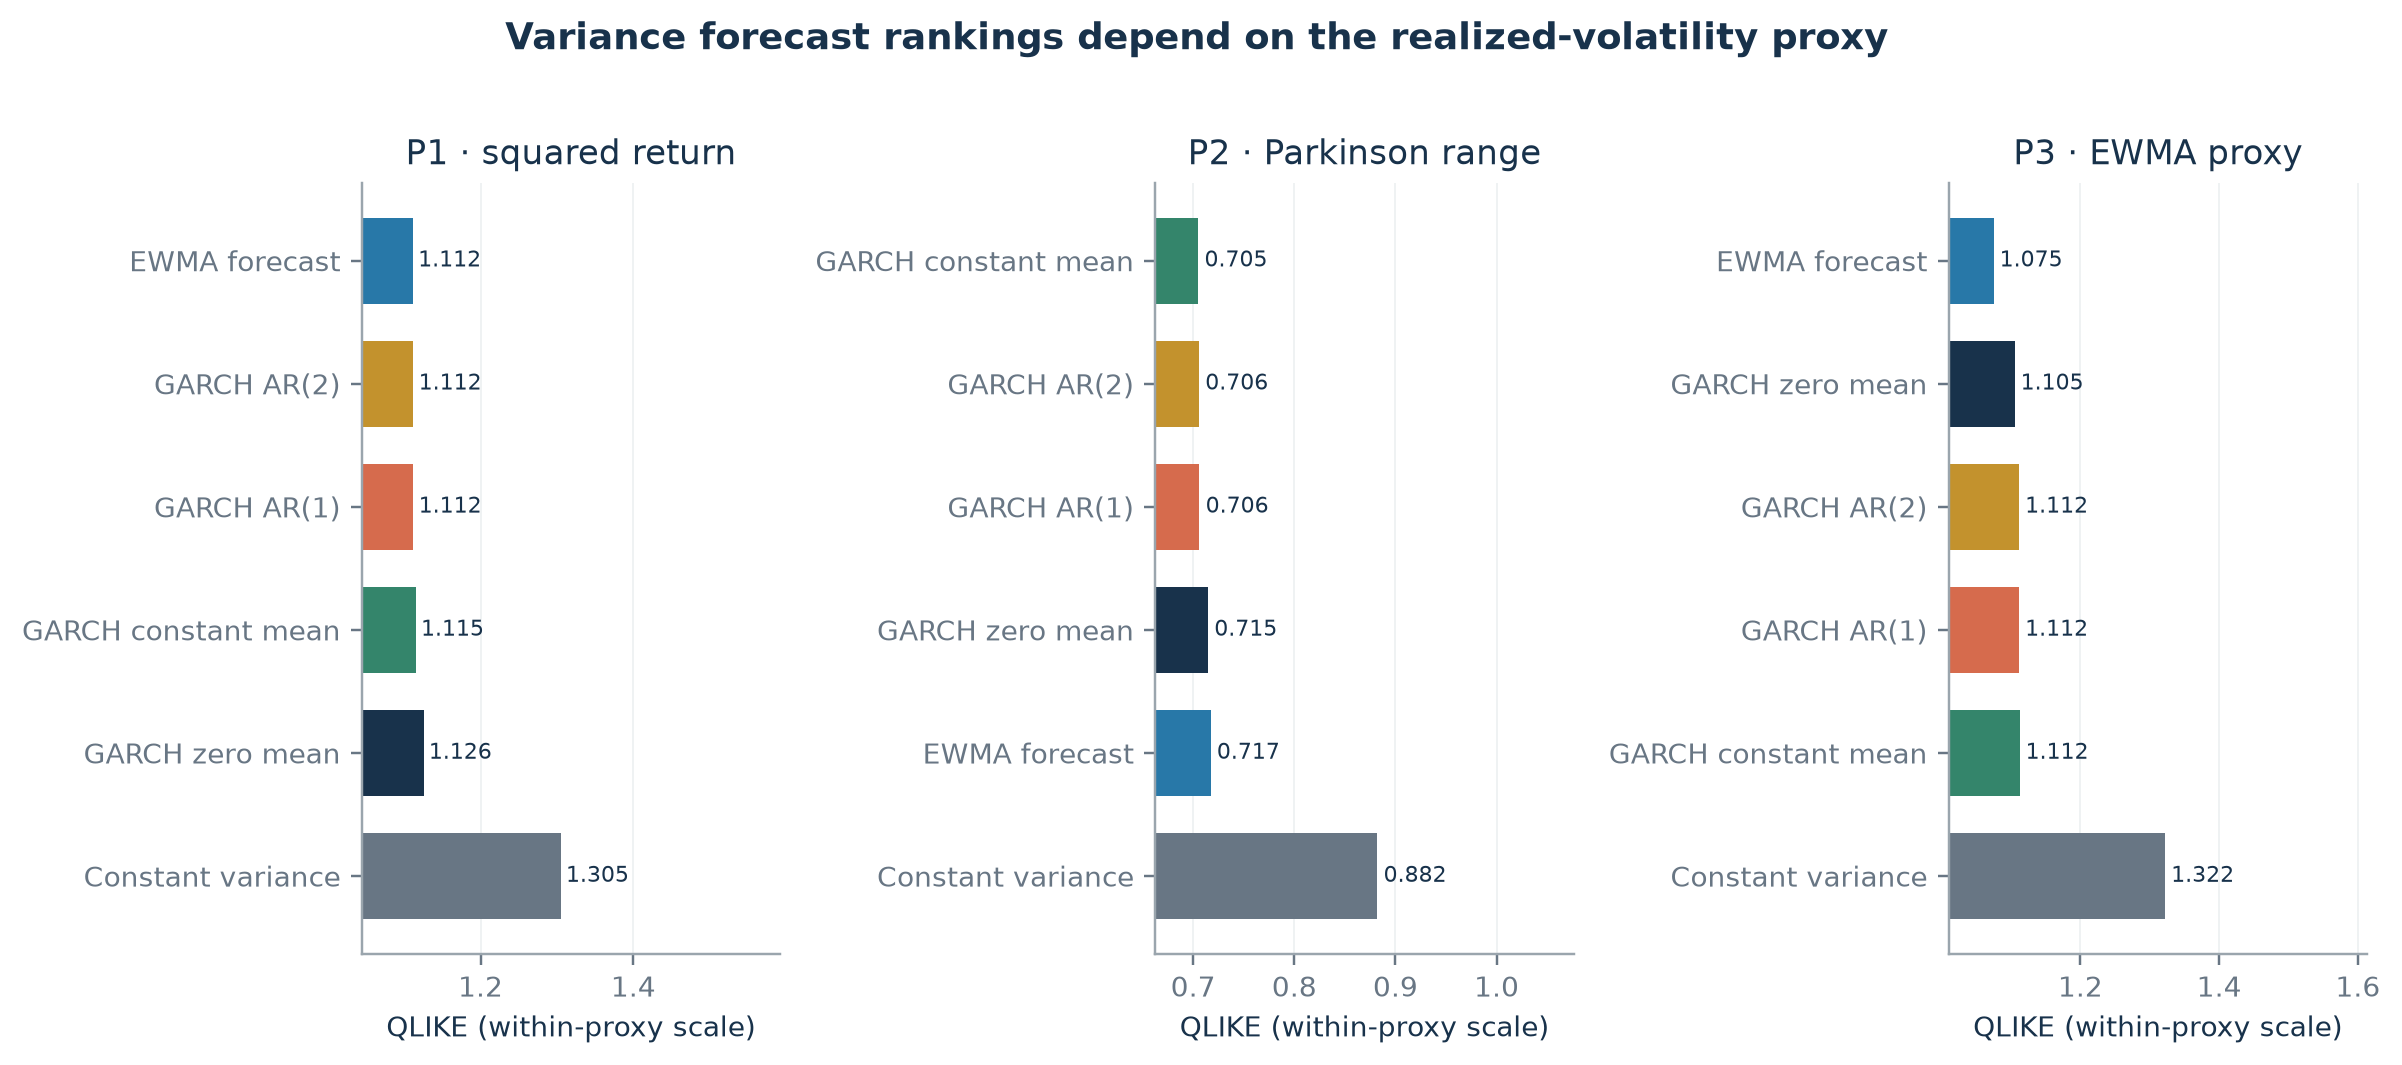
\includegraphics[width=\linewidth]{fig4_qlike_by_proxy.png}
\caption{Validation QLIKE rankings for the three registered realized-variance proxies. Lower is
better within a panel. Do not compare the numerical levels across panels: proxy definitions and
noise differ.}
\label{fig:qlike}
\end{figure}

EXP-004-S1 was pre-registered after the unconstrained fit reported
$\omega+\alpha+\beta>1$. The implementation forced that registered sum below one. All four
optimizations converged at its boundary; log likelihood fell by 1.46--1.84 relative to the
corresponding unconstrained fit. Under the conventional coefficient sum, the constrained fits
have $\alpha+\beta$ around 0.972--0.973. The AR(1)/AR(2) QLIKE ordering swaps, while every
candidate remains better than B1 and worse than B2 on P1. The predeclared rule therefore marked
the result MATERIAL. In light of the units issue, this sensitivity is best read as showing that
the near-tied AR(1)/AR(2) variance ordering depends on the imposed restriction; it is not evidence
that the unconstrained model violates the canonical GARCH finite-variance condition.

\subsection{EXP-005 through EXP-008: validation}
\begin{center}
\begin{tabular}{lrr}
\toprule
Forecast & RMSE & MAE\\
\midrule
Zero & 1.161796 & 0.863599\\
Training mean & 1.161796 & 0.863793\\
Constant GARCH mean & 1.163701 & 0.865138\\
AR(1)-GARCH mean & 1.166885 & 0.869240\\
AR(2)-GARCH mean & 1.166600 & 0.868866\\
PatchTST & 1.295198 & 1.000554\\
Validation-fitted combination & 1.161585 & 0.863545\\
\bottomrule
\end{tabular}
\end{center}
The comparison uses the same 603 validation dates. PatchTST does not beat zero or any classical
mean candidate. The combination's tiny RMSE improvement is validation-selected and should not
be interpreted as a stable gain. In the HAC DM comparisons, zero/training mean strongly
outperform PatchTST in squared loss; pairwise differences among the close classical/constant
baselines are not interpreted from point estimates alone. Encompassing regressions for
AR(1)+PatchTST and AR(2)+PatchTST give joint-signal $p$-values 0.983 and 0.992. Constant forecast
combinations with an intercept are rank deficient and reported as not identified.

Among the 15 two-forecast convex combinations, zero and training mean produce the best
validation RMSE. The fitted weights are 0.499943 and 0.500057. Since both forecasts are
constant through the validation period, their combination is also constant, near 0.02214
percentage points. The small score gain is a selected intercept adjustment, not evidence that
the pair captures changing return dynamics. This distinction matters: fitting a validation mean
and discovering out-of-sample predictive information are different achievements.

The encompassing regression is
$y_t=c+b_Af_{A,t}+b_Bf_{B,t}+u_t$, with Newey--West standard errors and lag 5. Because zero,
training mean, and the constant-mean GARCH forecast are constant series, regressions involving
them are often rank deficient with the intercept. Those coefficients are not identified and are
not reported as if they were estimable. The three full-rank regressions have joint HAC Wald
$p$-values 0.452 (AR(1)+AR(2)), 0.983 (AR(1)+PatchTST), and 0.992 (AR(2)+PatchTST). Large
$p$-values mean this sample does not reject the zero-coefficient null; they do not prove that
both forecasts contain no information.

The validation DM test for zero minus PatchTST has mean squared-loss difference $-0.32777$
percentage-point squared, 95\% HAC interval $[-0.43863,-0.21690]$, and
$p=1.06\times10^{-8}$. Training mean versus PatchTST is also $-0.32777$
($p=1.29\times10^{-8}$), and AR(1) versus PatchTST is $-0.31592$
($p=3.47\times10^{-8}$). Negative values favor the first model. These unadjusted tests provide
strong validation-period evidence against this PatchTST run; multiplicity remains a limitation.

The PatchTST RMSE is 11.5\% higher than zero on validation. This is not a near miss: the model
loses across RMSE and MAE, and the squared-loss DM comparison favors zero. It remains a result
for one predeclared architecture and a single validation period. Figure~\ref{fig:rmse-partitions}
shows both the large PatchTST gap and how close the classical alternatives remain.

\begin{figure}[htbp]
\centering
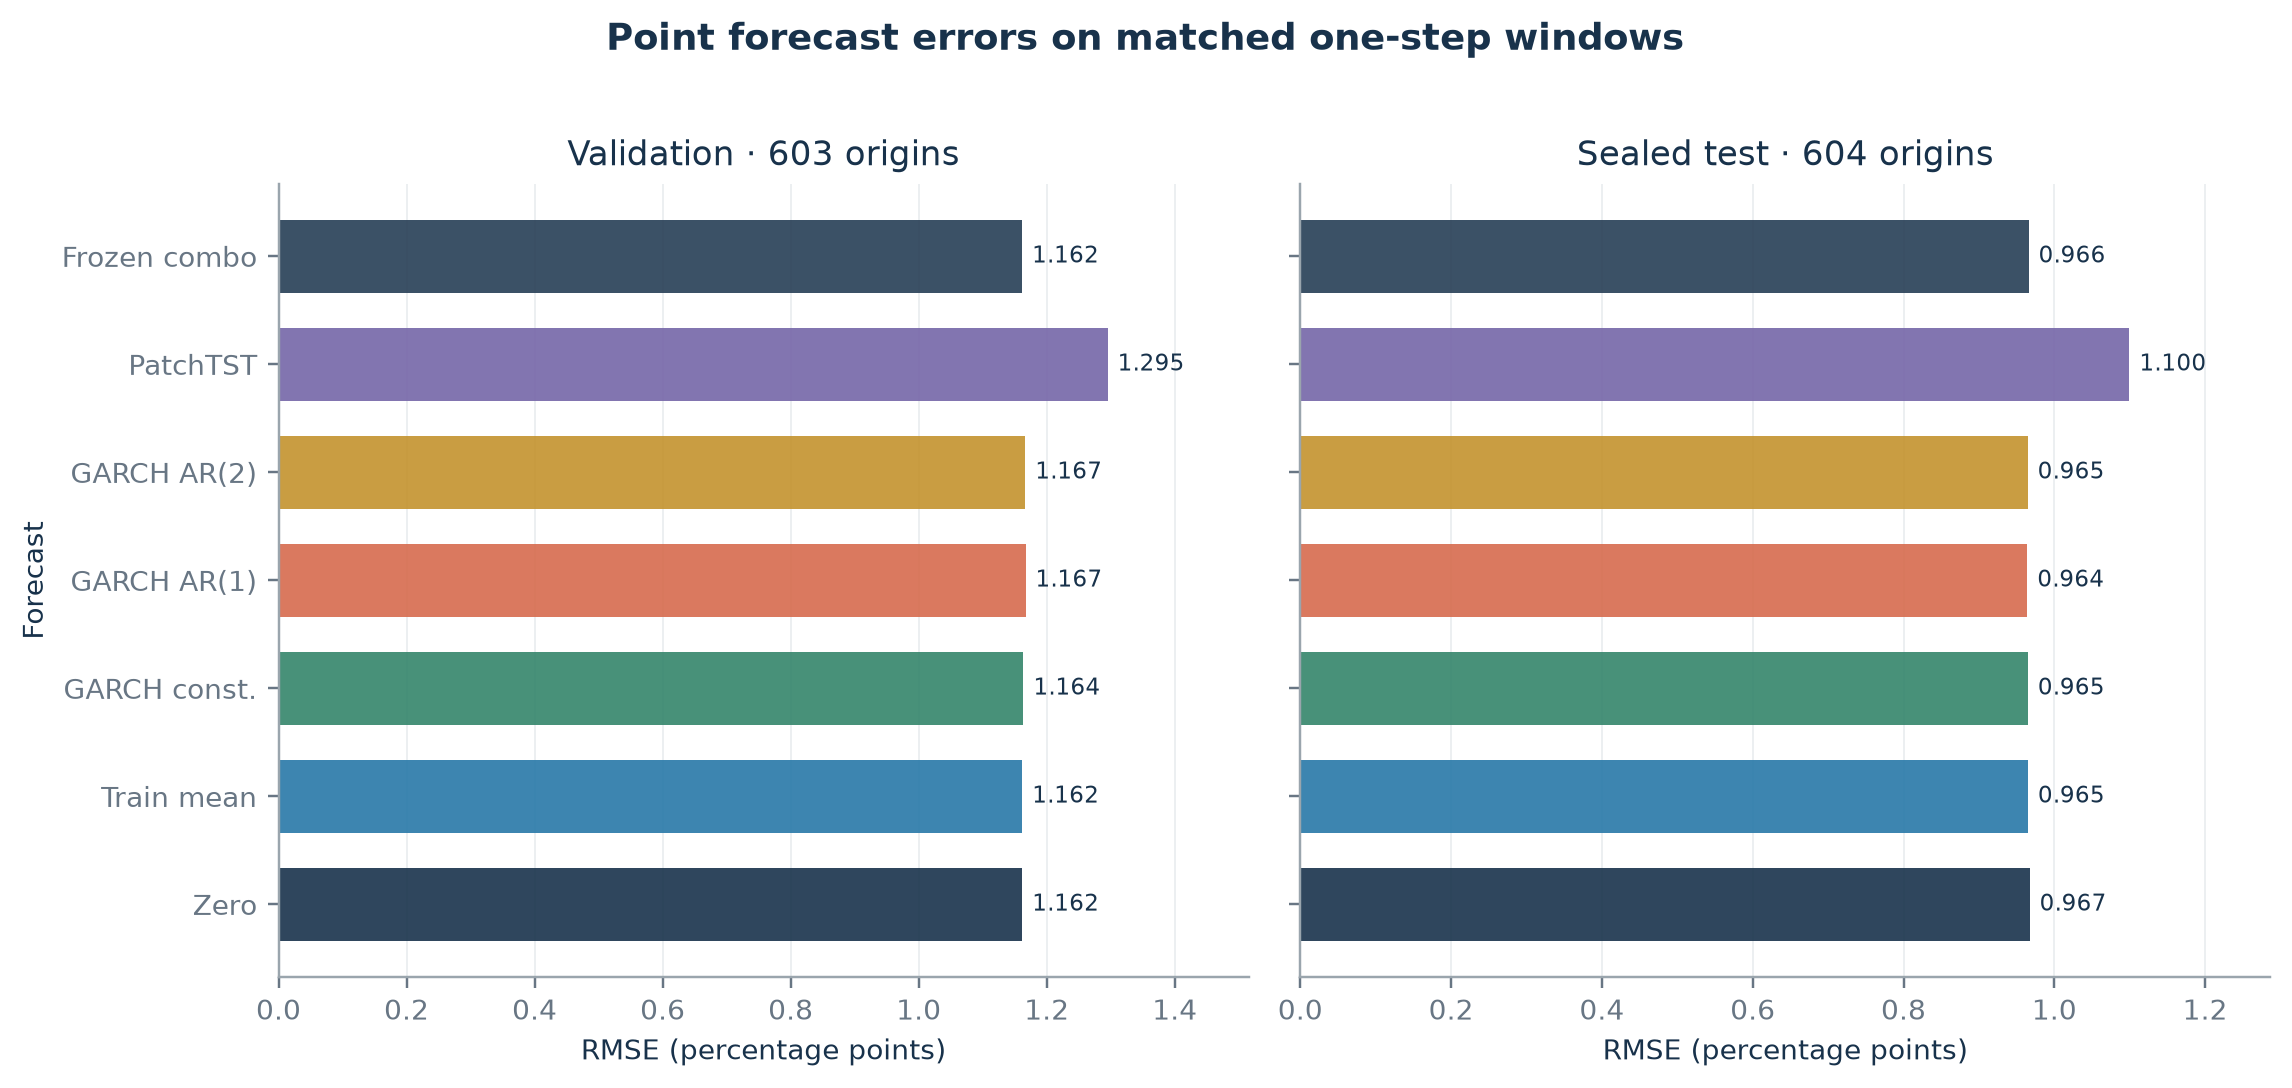
\includegraphics[width=0.98\linewidth]{fig3_rmse_validation_test.png}
\caption{RMSE on matched one-step origins in validation and test. Values use percentage-point
returns. The test panel is an ex-post display of the single frozen EXP-009 run and did not feed
back into model choice.}
\label{fig:rmse-partitions}
\end{figure}

\begin{figure}[htbp]
\centering
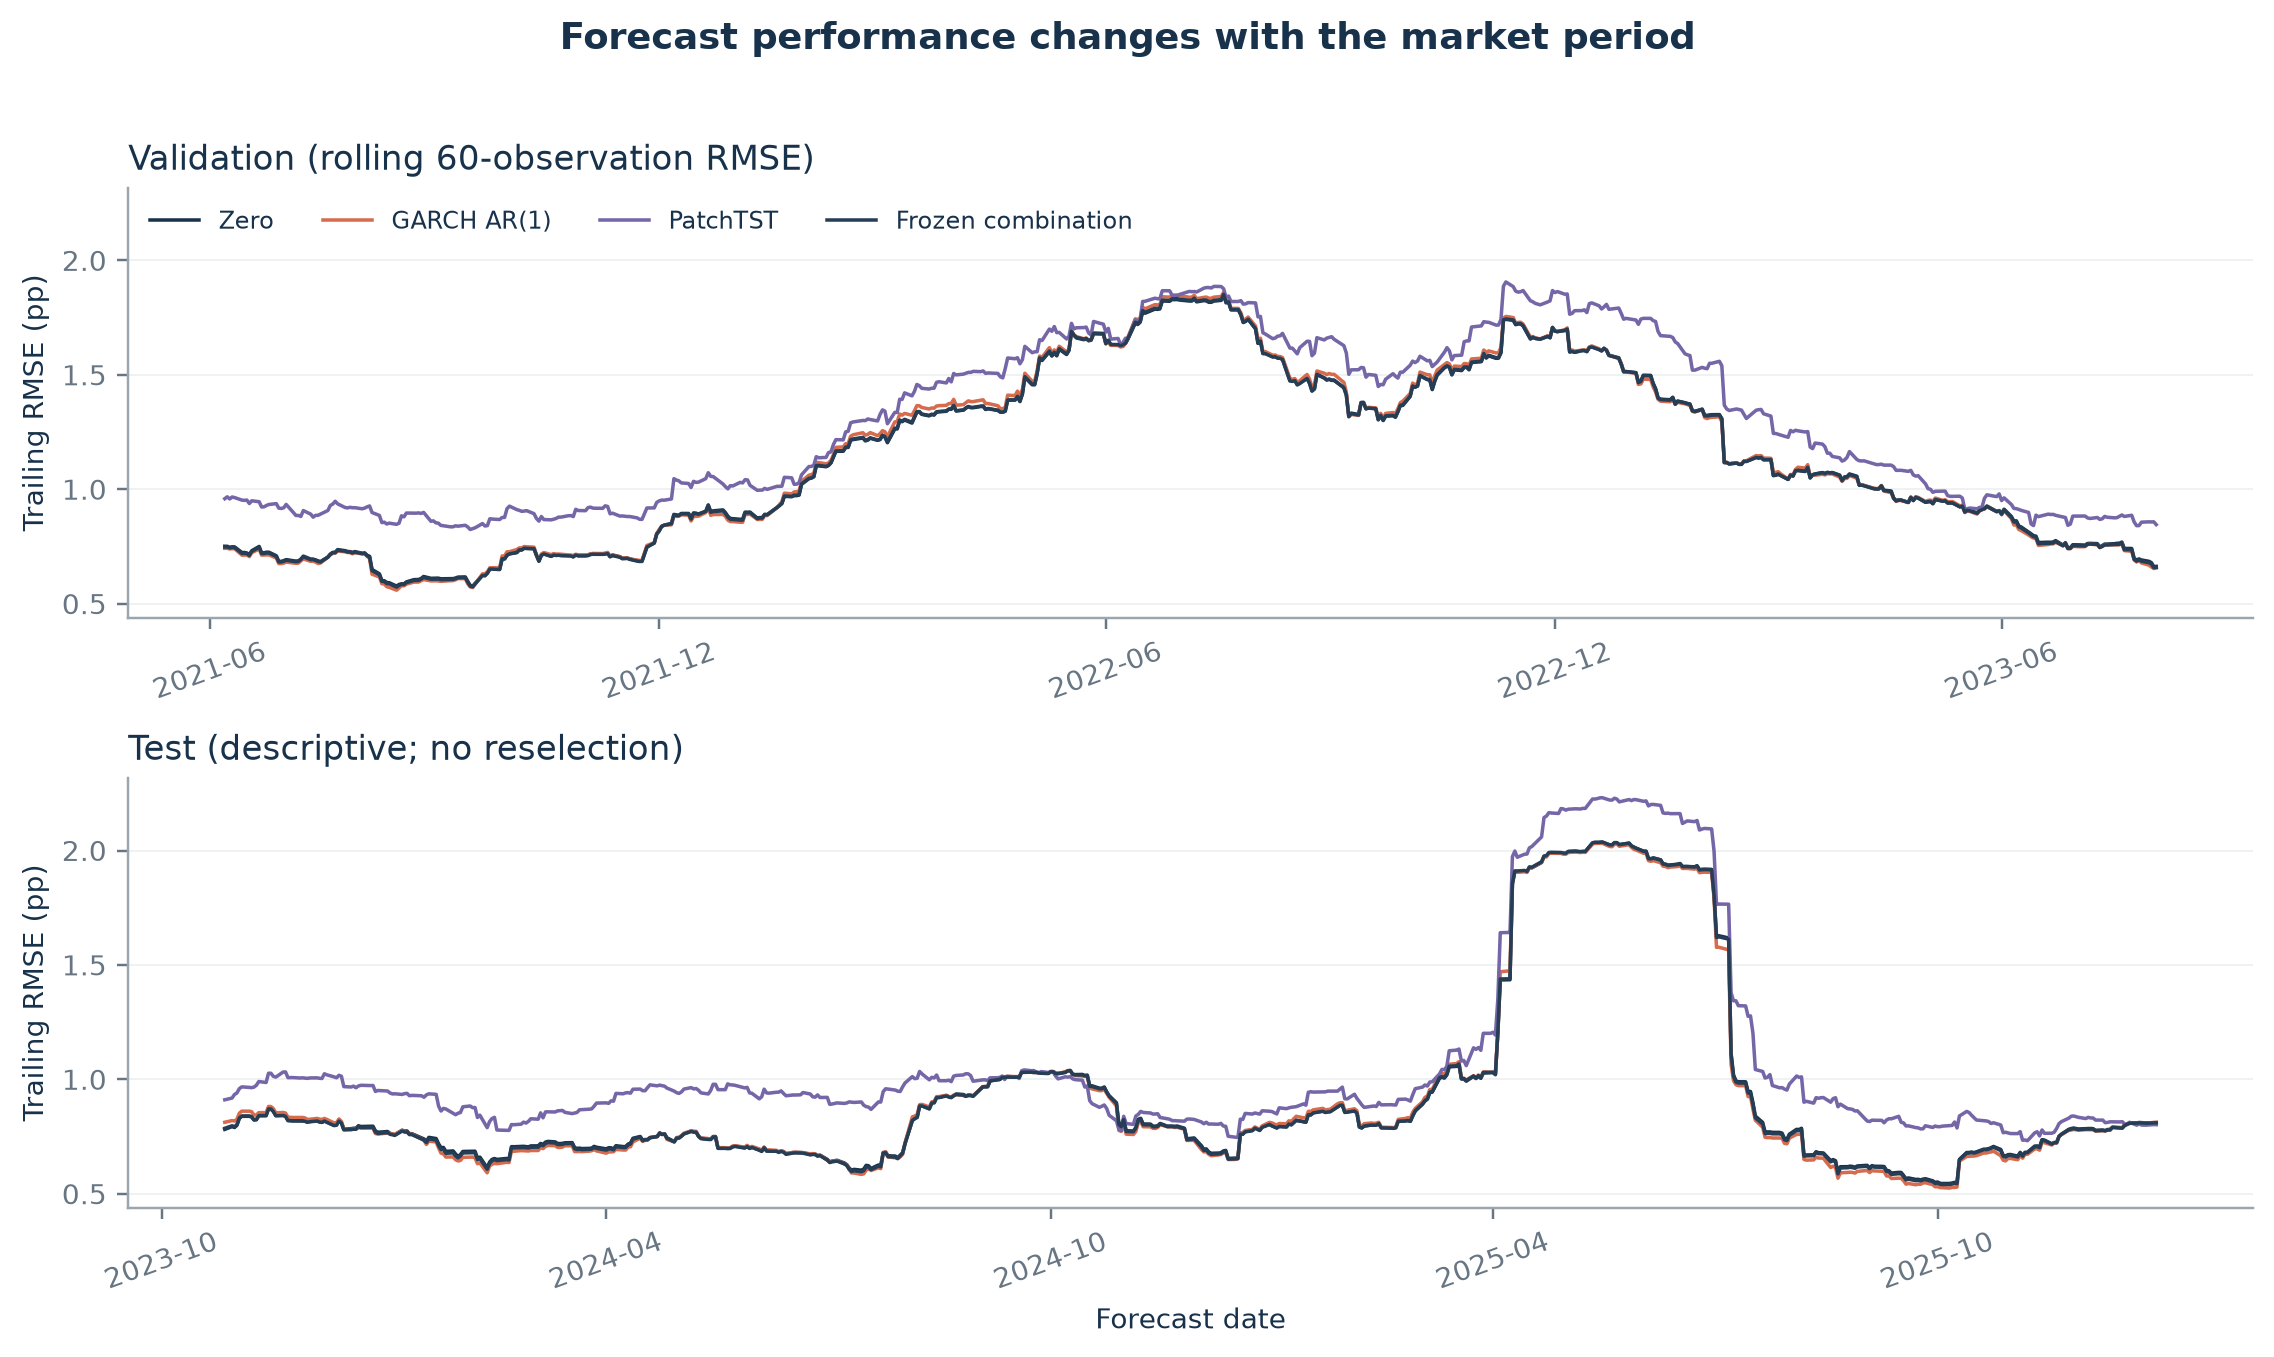
\includegraphics[width=0.98\linewidth]{fig6_rolling_rmse.png}
\caption{Trailing 60-observation RMSE for selected validation forecasts and the frozen test
forecasts. Aggregate loss is not uniform through time. The test panel is descriptive and was
not used for model selection.}
\label{fig:rolling-rmse}
\end{figure}

\subsection{EXP-009: sealed test}
The committed freeze selected the validation-fitted zero/training-mean combination as primary,
with weights fixed at 0.499943/0.500057. The selected single reference was training mean. The
exact PatchTST checkpoint hash, scaler, candidate list, target units, split dates, and analysis
method are in \texttt{docs/freeze\_manifest.json}. All test results below are from one run only.

\begin{center}
\begin{tabular}{lrr}
\toprule
Forecast & RMSE & MAE\\
\midrule
Zero & 0.967302 & 0.652373\\
Training mean & 0.965081 & 0.647674\\
Constant GARCH mean & 0.964965 & 0.645014\\
AR(1)-GARCH mean & 0.964290 & 0.646271\\
AR(2)-GARCH mean & 0.964722 & 0.646694\\
PatchTST & 1.099655 & 0.785724\\
Frozen combination (primary) & 0.965939 & 0.649630\\
\bottomrule
\end{tabular}
\end{center}
AR(1) has the lowest test RMSE point estimate, 0.964290; the frozen combination is 0.965939.
The primary HAC DM test of combination versus AR(1) has $p=0.802$ and a confidence interval
that includes zero. The combination also is not significantly different from zero ($p=0.104$)
or training mean ($p=0.307$). It has lower squared loss than PatchTST ($p=1.25\times10^{-5}$).
Therefore, the test does not support a meaningful performance separation among the simple and
classical forecasts, but it does favor the frozen combination over this PatchTST model. The
test ranking was not used to alter the frozen system.

\begin{table}[htbp]
\centering\small
\caption{EXP-009 primary Diebold--Mariano contrasts. Loss difference is frozen combination
minus comparator under squared error; negative favors the combination.}
\label{tab:test-dm}
\begin{tabular}{lrrr}
\toprule
Comparator & Mean difference (pp$^2$) & 95\% HAC interval & $p$-value\\
\midrule
Zero & $-0.002636$ & [$-0.005813$, $0.000541$] & 0.104\\
Training mean & $0.001656$ & [$-0.001521$, $0.004832$] & 0.307\\
GARCH constant & $0.001880$ & [$-0.008187$, $0.011947$] & 0.714\\
GARCH AR(1) & $0.003183$ & [$-0.021707$, $0.028072$] & 0.802\\
GARCH AR(2) & $0.002349$ & [$-0.022244$, $0.026942$] & 0.851\\
PatchTST & $-0.276203$ & [$-0.399225$, $-0.153182$] & $1.25\times10^{-5}$\\
\bottomrule
\end{tabular}
\end{table}
Figure~\ref{fig:test-dm} shows the same contrasts. Classical forecast intervals include zero;
the PatchTST interval lies below zero, favoring the frozen combination under squared loss. The
test does not support a reliable separation between the primary system and the small RMSE
ordering among classical forecasts.

\begin{figure}[htbp]
\centering
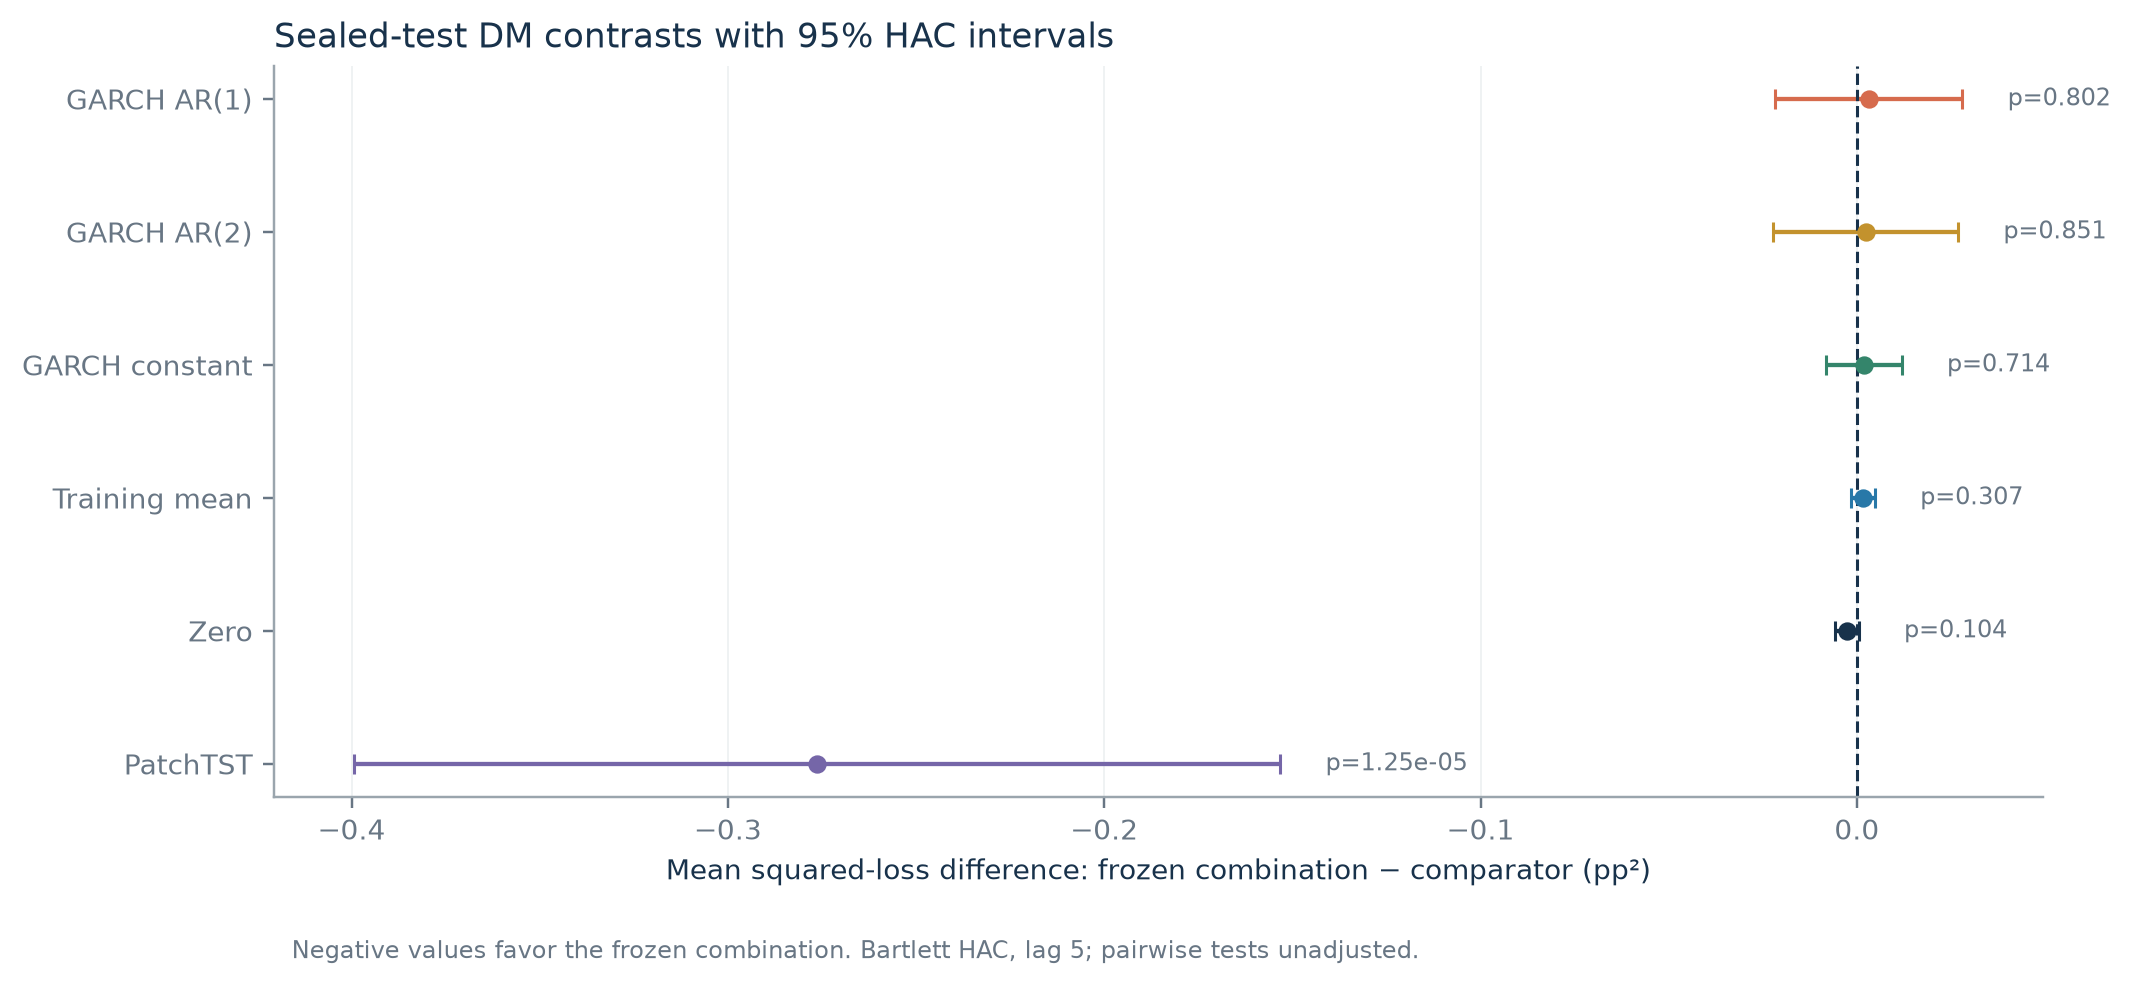
\includegraphics[width=0.98\linewidth]{fig7_test_dm_intervals.png}
\caption{Primary sealed-test DM contrasts with Bartlett HAC intervals. Negative differences
favor the frozen combination. The interval for PatchTST excludes zero; intervals for the simple
and classical forecasts include zero. Pairwise inference is not multiplicity adjusted.}
\label{fig:test-dm}
\end{figure}

\section{Interpretation guide}
\begin{enumerate}
\item \textbf{Check units first.} A return of 1 means one percentage point of log return, not a
   decimal return of 1. Variances and proxies are in squared percentage points.
\item \textbf{Separate fit diagnostics from forecast performance.} ADF, Ljung--Box, ARCH LM,
   convergence, and persistence describe assumptions/residuals. Validation/test RMSE and MAE
   describe point forecast error.
\item \textbf{Read loss differences with their sign.} In this report $d=L_A-L_B$; negative means
   A's average loss is smaller. Check the CI and HAC p-value before claiming a distinction.
\item \textbf{Respect the partition.} Validation selected the combination; its validation score
   is optimistic. The test is the confirmatory result and must not be reused to tune.
\item \textbf{Treat proxy-sensitive volatility results conditionally.} QLIKE rankings can vary
   with the proxy; compare only within a given proxy and disclose the persistence sensitivity.
\item \textbf{Keep scope narrow.} One index, one daily horizon, one validation/test period, one
   small PatchTST configuration, and unadjusted pairwise tests do not establish universal claims.
\end{enumerate}

\section{Implementation, verification, and reproducibility}
The code separates return loading/splitting, classical fits, Transformer data/model/training, and
evaluation. The main evaluation modules are:
\begin{itemize}
\item \texttt{compare.py} and \texttt{combination.py};
\item \texttt{encompassing.py} and \texttt{dm\_test.py};
\item \texttt{final\_test.py}.
\end{itemize}
Tests cover provenance, chronological splits, forecast alignment, leakage, model shapes/checkpoint
reload, metric arithmetic, GARCH constraints, convex weights, rank-deficient encompassing
designs, and DM arithmetic.

Several implementation failures were useful rather than cosmetic. The first PatchTST run failed
because PyTorch interpreted a one-dimensional temporal patch argument as a two-dimensional
16-by-16 image kernel. The model now adds singleton height and slides a 1-by-16 kernel along the
time axis. Focused leakage tests also exposed exact-float comparisons between float64 source
arrays and intentionally float32 model windows; those assertions now use explicit tolerances.
The training runner originally built scaled inputs through the full data series. It was corrected
to construct origins only through the validation endpoint, leaving test inputs outside the
EXP-005 path. The saved Phase 2 state dictionary is SHA256-checked at final inference.

The first EXP-007 encompassing run encountered a singular design and then an indexing error when
the regression helper omitted an intercept for constant forecast columns. The final implementation
forces the intercept, checks matrix rank before estimation, and records unidentified regressions
explicitly. This matters because a constant prediction and an intercept are the same regressor.

\subsection{Artifact map and reproducible commands}
Every run uses a unique timestamped ID. The central artifacts are:
\begin{itemize}
\item EXP-003 fit/diagnostics JSON and 603-row validation forecast CSV under
  \path{results/tables/} and \path{results/forecasts/};
\item EXP-004 QLIKE matrix and proxy-evaluation JSON; EXP-004-S1 constrained-fit JSON;
\item EXP-005 config, learning history, validation forecast, and frozen `.pt` checkpoint;
\item EXP-006 matched-date score table; EXP-007 combination and encompassing results;
\item EXP-008 paired DM results; EXP-009 single test forecast CSV and score JSON;
\item seven report figures under \path{paper/figures/}.
\end{itemize}
The prose is a readable account; exact parameter standard errors, $p$-values, convergence
messages, forecast origins, and all model-pair metrics remain in the machine-readable artifacts.
The experiment register, decision log, freeze manifest, and saved outputs provide the
reproducibility record for the experiments described here.

Run from the repository root:
\begin{lstlisting}
export UV_CACHE_DIR=/tmp/solitons-uv-cache
export MPLCONFIGDIR=/tmp/solitons-mpl
uv run python -m src.experiments.complete_retro
uv run python -m src.transformer.train
uv run python -m src.evaluation.compare
uv run python -m src.evaluation.combination
uv run python -m src.evaluation.dm_test
uv run python paper/make_figures.py
uv run pytest -q
\end{lstlisting}
The final-test command is intentionally one-time after the freeze commit:
\begin{lstlisting}
uv run python -m src.evaluation.final_test
\end{lstlisting}
The full suite passes 71 tests. It emits 16 statsmodels FutureWarnings about a future diagnostic
return type and 7 PyTorch nested-tensor fast-path warnings; no warnings were suppressed.
Machine-readable artifacts and experiment records in \texttt{results/} and \texttt{docs/} retain
the detailed values, parameters, warnings, and run IDs.

\section{Discussion, limitations, and conclusion}
The mean-return evidence is consistent across model families: the training sample has enormous
dependence in squared returns and very heavy tails, yet the conditional-mean forecasts are hard to
improve over a constant near zero. That combination is not paradoxical. Predictable volatility
does not imply predictable return direction or mean. The GARCH layer can model the scale of
surprises while the mean remains close to zero.

The variance results also illustrate why model comparison is measurement dependent. B2 EWMA
wins on the squared-return and smoothed EWMA proxies, while the GARCH models win against B2 on
the Parkinson range proxy. No one proxy is a noiseless view of latent variance, and P3 is
structurally related to the EWMA recursion used by B2. The proxy-specific conclusion is more
credible than declaring one universal volatility winner.

The canonical GARCH coefficient sums $\alpha+\beta$ are below one but close to the boundary.
The registered sum including $\omega$ exceeds one because it combines parameters with different
units. This report corrects the interpretation while preserving the original log, fit outputs,
and constrained sensitivity. The constrained exercise remains useful as a predeclared
specification sensitivity, but it should not be cited as the standard stationarity-constrained
GARCH estimate.

The central neural result is negative but bounded. The chosen PatchTST is substantially worse
than zero in validation and worse than the frozen combination in the final test. This does not
show that all Transformers fail: the model is univariate, deliberately small, untuned, and
trained for one-step squared-error loss. It shows that this specific, reproducible configuration
did not earn its complexity on these data.

The frozen combination's validation gain is only 0.000211 RMSE points and disappears as a
statistically detectable gain on test. Its test loss is close to zero, training mean, and the
four GARCH mean forecasts. AR(1) has the smallest test RMSE point estimate, but the combination
versus AR(1) DM interval spans zero widely. The practical conclusion is not that the combination
won; rather, several simple/classical forecasts are difficult to distinguish over this one test
window, while the tested PatchTST is clearly worse under squared loss.

Five limits constrain the claim. First, one equity index and one split do not represent all
markets or regimes. Second, a single validation period makes hyperparameter or combination
selection noisy. Third, pairwise HAC tests are not multiplicity adjusted. Fourth, realized
variance proxies are noisy and not mutually interchangeable. Fifth, the test run is one sealed
evaluation and cannot be reused for further tuning. The RMSE target of a 15\% Transformer
improvement was a goal, not an observed result. Nothing here establishes economic value after
transaction costs or trading constraints.

In short: the project finds strong volatility clustering, little practical mean-forecast gain
from the tested AR terms, proxy-sensitive variance rankings, and no validation/test advantage
for this PatchTST. The most defensible result is that no deep-forecasting gain was demonstrated
for this one-step return task under the frozen protocol.

\appendix
\section{Full EXP-003 coefficient estimates}
Table~\ref{tab:coefficients} gives the principal point estimates. The exact standard errors,
Wald statistics, and $p$-values for every coefficient are retained in this machine-readable
EXP-003 JSON artifact:
\begin{quote}\small\url{results/tables/exp003_garch_mean_spec_20261116T113919Z_6cb9.json}\end{quote}

\begin{table}[htbp]
\centering\small
\caption{EXP-003 GARCH(1,1)-Student-$t$ parameter estimates on training data.}
\label{tab:coefficients}
\begin{tabular}{lrrrrrrr}
\toprule
Mean & Mean intercept & $\phi_1$ & $\phi_2$ & $\omega$ & $\alpha$ & $\beta$ & $\nu$\\
\midrule
Zero & -- & -- & -- & 0.025581 & 0.172995 & 0.817852 & 5.1015\\
Constant & 0.092275 & -- & -- & 0.026690 & 0.187191 & 0.806172 & 4.9015\\
AR(1) & 0.099490 & $-0.066310$ & -- & 0.025907 & 0.184328 & 0.809776 & 4.8343\\
AR(2) & 0.100166 & $-0.066567$ & $-0.005660$ & 0.025869 & 0.184181 & 0.809937 & 4.8339\\
\bottomrule
\end{tabular}
\end{table}
The negative lag-one coefficient is small relative to return volatility. The lag-two coefficient
in AR(2) is close to zero. Estimated $\nu$ between 4.83 and 5.10 indicates materially heavier
tails than a Gaussian distribution, while the variance coefficients imply slowly decaying
volatility shocks.

\begin{longtable}{llrrr}
\caption{EXP-003 coefficient estimates, asymptotic standard errors, and two-sided Wald $p$-values.}\label{tab:full-inference}\\
\toprule Specification & Parameter & Estimate & Std. error & $p$-value\\
\midrule
\endfirsthead
\toprule Specification & Parameter & Estimate & Std. error & $p$-value\\
\midrule
\endhead
Zero & $\omega$ & 0.025581 & 0.006010 & $2.08\times10^{-5}$\\
Zero & $\alpha_1$ & 0.172995 & 0.021538 & $9.59\times10^{-16}$\\
Zero & $\beta_1$ & 0.817852 & 0.019193 & $<10^{-12}$\\
Zero & $\nu$ & 5.101463 & 0.500361 & $2.08\times10^{-24}$\\
Constant & $\mu$ & 0.092275 & 0.011636 & $2.19\times10^{-15}$\\
Constant & $\omega$ & 0.026690 & 0.005987 & $8.27\times10^{-6}$\\
Constant & $\alpha_1$ & 0.187191 & 0.023567 & $1.97\times10^{-15}$\\
Constant & $\beta_1$ & 0.806172 & 0.020150 & $<10^{-12}$\\
Constant & $\nu$ & 4.901547 & 0.449343 & $1.05\times10^{-27}$\\
AR(1) & $c$ & 0.099490 & 0.012164 & $2.85\times10^{-16}$\\
AR(1) & $\phi_1$ & $-0.066310$ & 0.018632 & 0.000372\\
AR(1) & $\omega$ & 0.025907 & 0.005892 & $1.10\times10^{-5}$\\
AR(1) & $\alpha_1$ & 0.184328 & 0.023458 & $3.91\times10^{-15}$\\
AR(1) & $\beta_1$ & 0.809776 & 0.019972 & $<10^{-12}$\\
AR(1) & $\nu$ & 4.834278 & 0.437173 & $2.00\times10^{-28}$\\
AR(2) & $c$ & 0.100166 & 0.012722 & $3.46\times10^{-15}$\\
AR(2) & $\phi_1$ & $-0.066567$ & 0.018628 & 0.000352\\
AR(2) & $\phi_2$ & $-0.005660$ & 0.020446 & 0.782\\
AR(2) & $\omega$ & 0.025869 & 0.005886 & $1.11\times10^{-5}$\\
AR(2) & $\alpha_1$ & 0.184181 & 0.023447 & $3.99\times10^{-15}$\\
AR(2) & $\beta_1$ & 0.809937 & 0.019951 & $<10^{-12}$\\
AR(2) & $\nu$ & 4.833923 & 0.436800 & $1.82\times10^{-28}$\\
\bottomrule
\end{longtable}
The mean intercepts in the AR fits are not the unconditional AR means; their lag coefficients
must also be considered. AR(2)'s second-lag coefficient is not statistically distinguishable
from zero in this fitted specification ($p=0.782$). These in-sample Wald tests are descriptive;
they do not replace the shared-date forecast comparison.

\section{The registered persistence sensitivity, read carefully}
For completeness, the EXP-004-S1 rule imposed the project diagnostic
$\omega+\alpha+\beta<1$. The constrained estimates converged very close to that boundary and
had likelihood reductions of 1.46--1.84 points. Standard errors and $p$-values were not computed
for the inequality-constrained estimates. Their canonical coefficient sums $\alpha+\beta$ were
0.972--0.973. The original predeclared MATERIAL verdict is retained in the experiment log; the
mathematical clarification here narrows what that verdict means. It signals sensitivity of a
near-tied variance ranking to the particular restriction, not proof that the unconstrained
GARCH coefficients violate $\alpha+\beta<1$.

\section{Numerical score examples}
Suppose on one date the actual return is $y=1.0$ pp, forecast A is $0.2$ pp, and forecast B is
$0.0$ pp. Their squared errors are $(1.0-0.2)^2=0.64$ and $(1.0-0.0)^2=1.00$ pp$^2$; the
one-date differential $L_A-L_B=-0.36$ favors A. A DM test averages these paired differences
over time and divides by a HAC standard error, so serial dependence affects the uncertainty,
not the definition of the sign.

For an RMSE interpretation, an RMSE of 1.0 pp is the square root of average squared error in
percentage-point units. It does not mean the forecast misses every date by exactly one point;
large errors receive more weight. That sensitivity to extremes is visible in the return
distribution and is one reason the GARCH variance model and Student-$t$ innovations are
considered.

\section*{Selected references}
\begin{itemize}
\item Bollerslev, T. (1986). Generalized autoregressive conditional heteroskedasticity.
  \emph{Journal of Econometrics}, 31(3), 307--327.
\item Diebold, F. X. and Mariano, R. S. (1995). Comparing predictive accuracy.
  \emph{Journal of Business \& Economic Statistics}, 13(3), 253--263.
  \url{https://doi.org/10.1080/07350015.1995.10524599}.
\item Harvey, D., Leybourne, S., and Newbold, P. (1997). Testing the equality of prediction mean
  squared errors. \emph{International Journal of Forecasting}, 13(2), 281--291.
\item Newey, W. K. and West, K. D. (1987). A simple, positive semi-definite, heteroskedasticity
  and autocorrelation consistent covariance matrix. \emph{Econometrica}, 55(3), 703--708.
\item Patton, A. J. (2011). Volatility forecast comparison using imperfect volatility proxies.
  \emph{Journal of Econometrics}, 160(1), 246--256.
  \url{https://doi.org/10.1016/j.jeconom.2010.03.034}.
\item Zhou, T. et al. (2023). A time series is worth 64 words: Long-term forecasting with
  Transformers. \emph{International Conference on Learning Representations}.
  \url{https://arxiv.org/abs/2211.14730}.
\end{itemize}

\end{document}
